\section{Problem E}
\textit{Perform time reversal in a MISO context for each set of 2 channel realizations (one from A and one from D). Calculate the average power delay profile of the equivalent channel and from that the delay spread. How does it compare to the delay spread calculated in B and C?}

Applying time reversal in a MISO fashion means to sum the autocorrelation functions (convolutions) of each of the received antenas (see last slide in page 4 of mm1).

\code{language=Matlab,caption = Time reversal in MISO fashion,label=cl:imp_resp_code,linerange={189-212},firstnumber=189}{code/mm1/mm1_pretty_solution_pretty_coments_Labels_and_DB.m}

The time reversed signal in a MISO fashion is shown in \figref{fig:ex_e_miso_2channels}

\begin{figure}
\centering
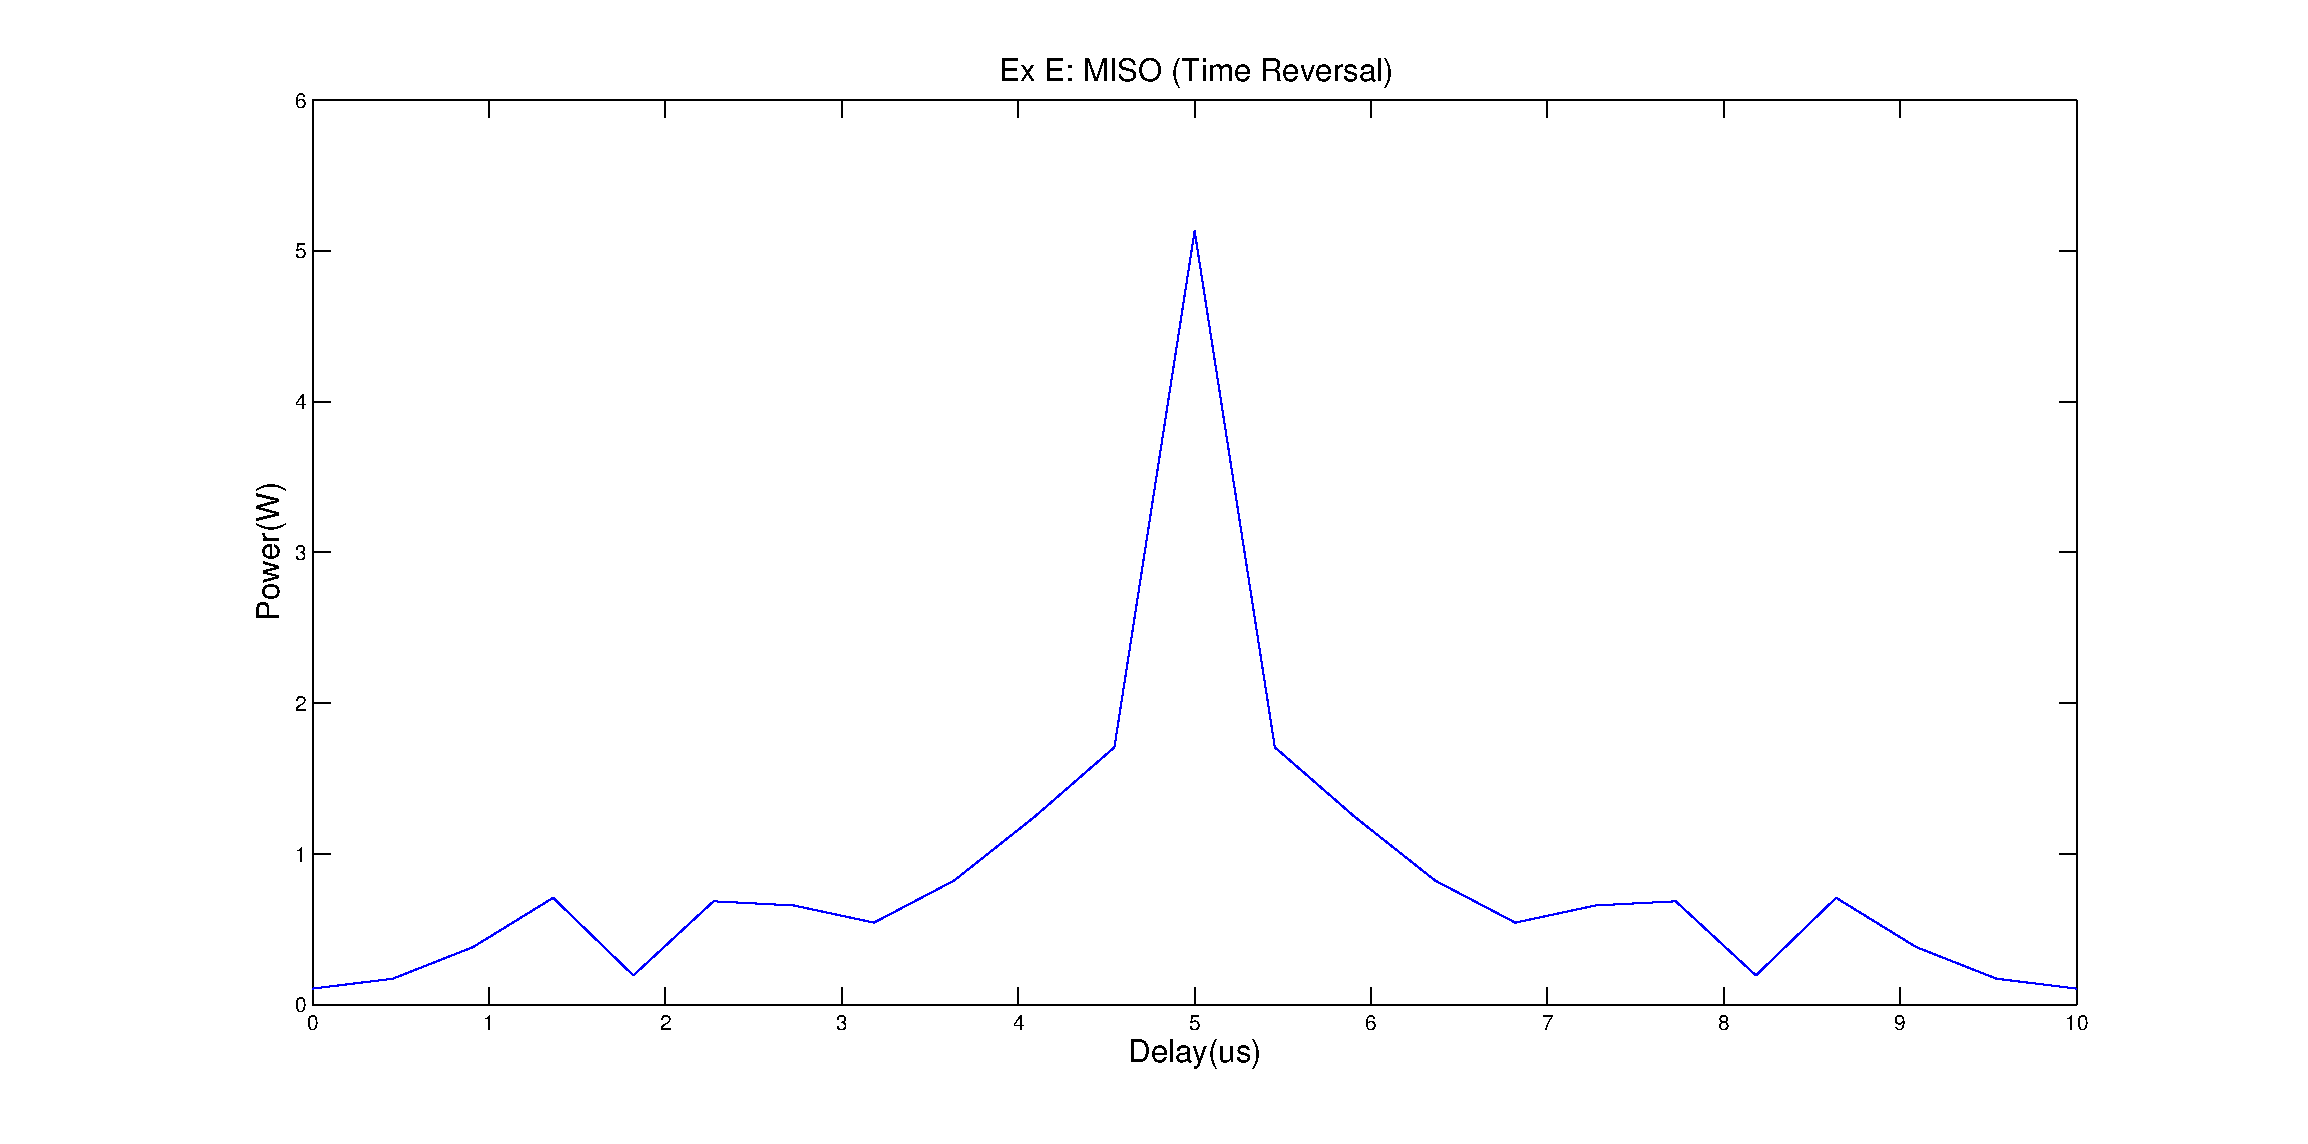
\includegraphics[width=9cm]{ex_e_miso_2channels.eps}
\caption{Impulse Response and PDP}\label{fig:ex_e_miso_2channels}
\end{figure}

As an extra, we decided to do the time reversal of the signal in a MISO fashion using 16 antennas instead of 2. The resulted time reversed signal is shown in \figref{fig:ex_e_miso_16channels}

\begin{figure}
\centering
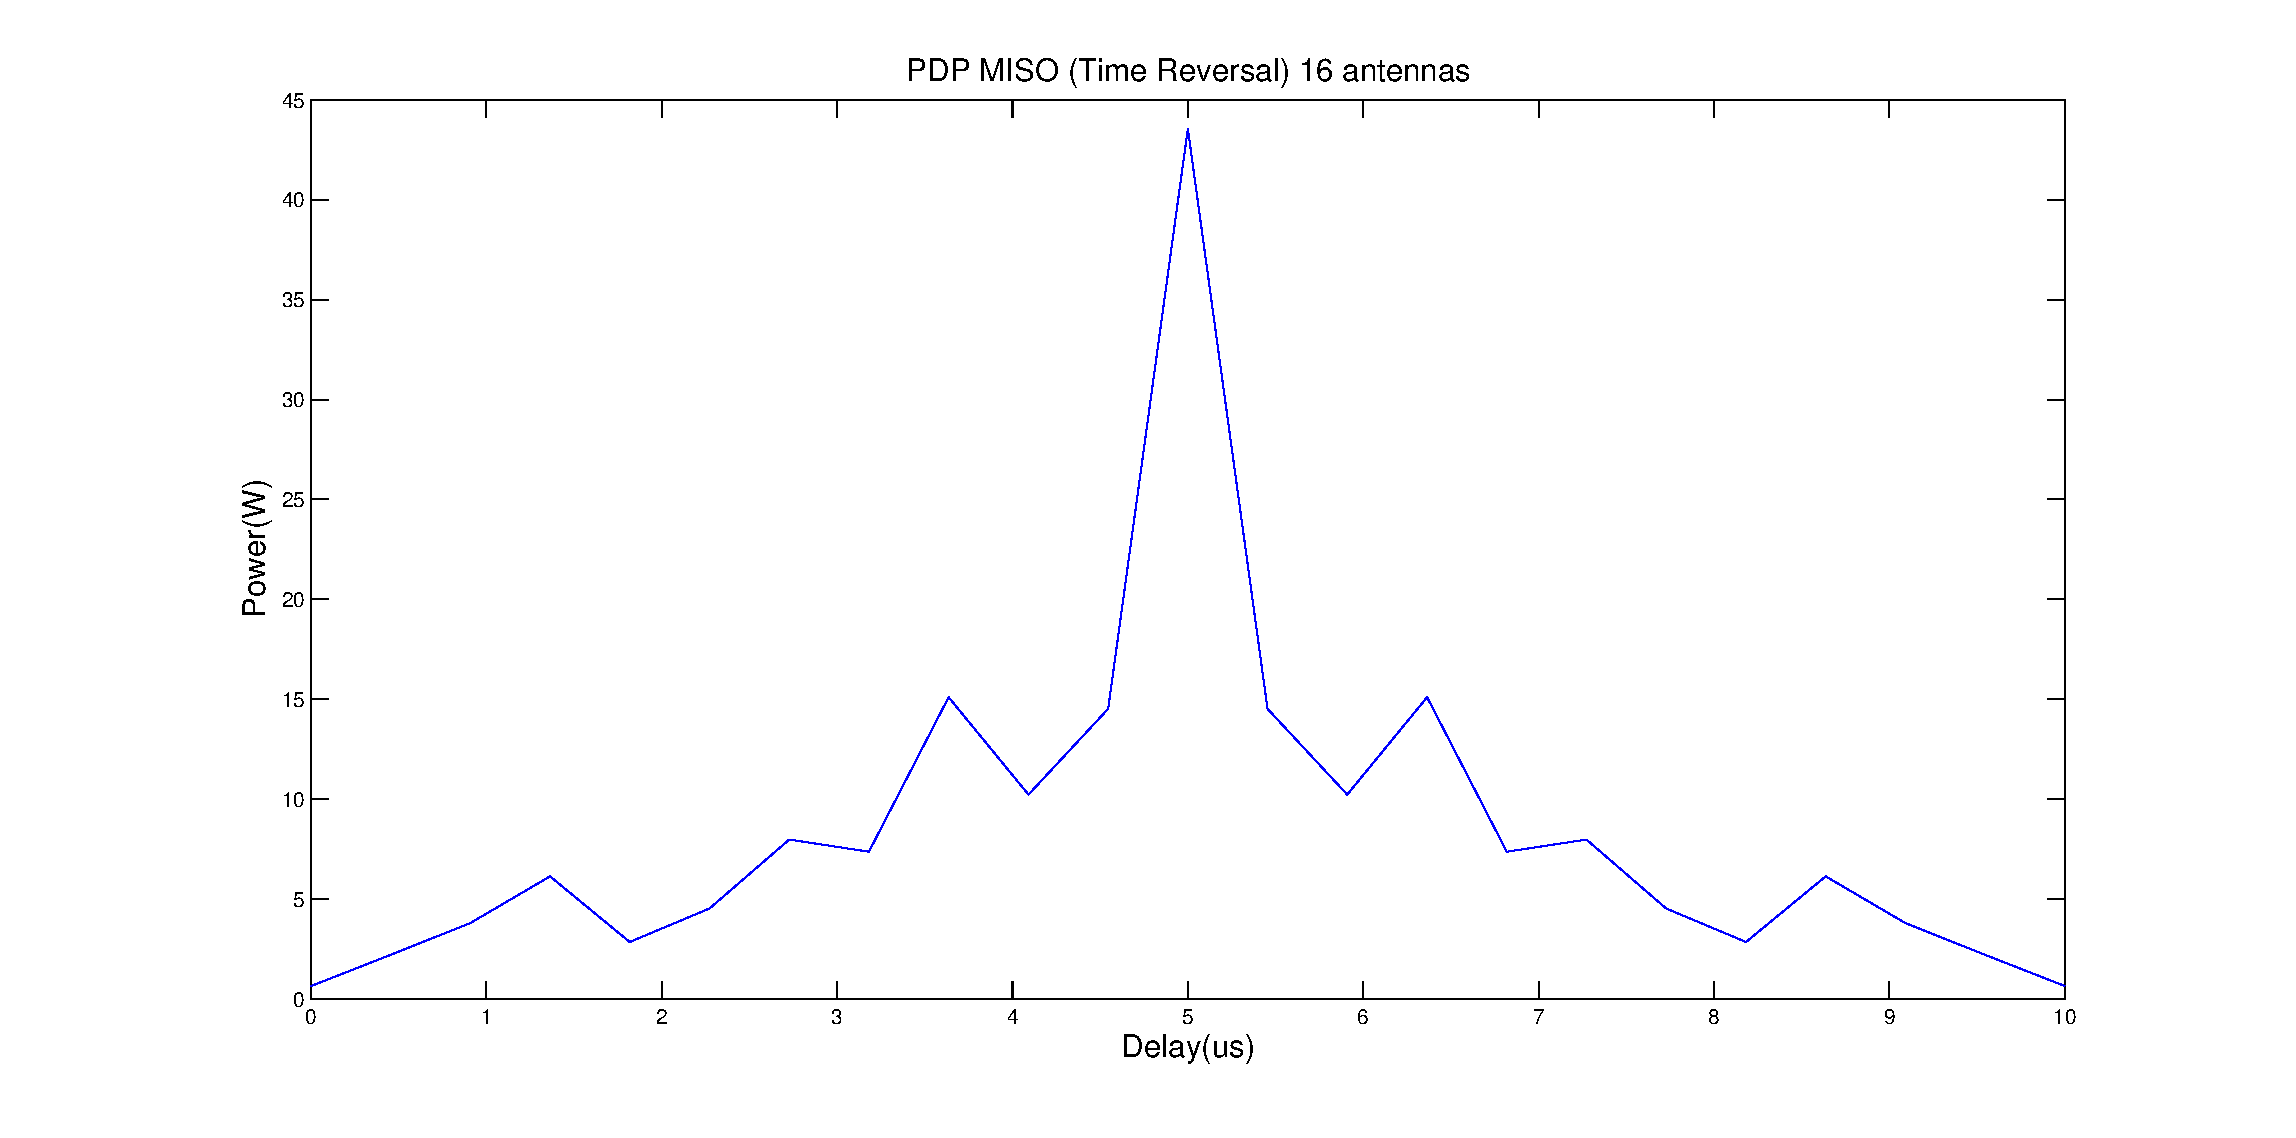
\includegraphics[width=9cm]{ex_e_miso_16channels.eps}
\caption{Impulse Response and PDP}\label{fig:ex_e_miso_16channels}
\end{figure}

In these cases the delay spread was similar to that calculated for one antenna.

In \tref{tab:power_del_spread} the power delay spread of all the calculated cases are reported.

\section{Making a table} 
\ptable{| p{10cm} | p{8cm} |}{ %
Case 							&	Delay spread [\SI{}{\micro\second}] 												\\ \hline
Taps from table 		        &	$1.026$											        \\ \hline
Several realizations of the channel 	        &	$1.024$										            \\ \hline
Time reversed signal							&	$1.753$	    							\\ \hline
Time reversed signal (MISO) 2 antennas			& 	$1.678$                           \\ \hline	
Time reversed signal (MISO) 16 antennas			        &	$1.753$ 	                        \\ \hline
}{Power delay spread for the different cases}{tab:power_del_spread}